\documentclass[twoside,openright]{uva-bachelor-thesis}

\usepackage{emptypage} % removes page numbers on empty twoside pages

% Fonts and input encoding
\usepackage[utf8]{inputenc}
\usepackage{ae,aecompl}
\usepackage{sourcecodepro}
\usepackage[T1]{fontenc}

% Random text
\usepackage{lipsum}
\setlipsumdefault{131}

% Bibliography
\usepackage[square,numbers]{natbib}
\usepackage[nottoc,numbib]{tocbibind}
\renewcommand\bibname{References}

% Figures and graphics
\usepackage{graphicx}
\usepackage{epstopdf}
\usepackage{float}
\usepackage{pgfplots} % plotting

% References
\usepackage{hyperref}
\hypersetup{pdfborder={0 0 0}} % remove borders around PDF links
\usepackage[noabbrev]{cleveref}
\crefdefaultlabelformat{#2#1#3}

% Remove leading paragraph indent
\usepackage{parskip}
\setlength{\parindent}{0pt}
\setlength{\parskip}{1.3ex plus 0.5ex minus 0.3ex}

% Captions
\usepackage[format=plain,labelfont=sf,bf,up,textfont=it,up]{caption}
\usepackage{subfig}

% Code formatting
\usepackage{color}
\usepackage{listings}

\lstdefinestyle{cstyle}{
	language=C++,
	escapeinside={\%*}{*)},
	morecomment=[l]{//},
	morecomment=[s]{/*}{*/},
	morekeywords={  abstract, event, new, struct,
		as, explicit, null, switch, base, extern, object, this,
		bool, false, operator, throw,
		break, finally, out, true, byte, fixed, override, try,
		case, float, params, typeof, catch, for, private, uint,
		char, foreach, protected, ulong, checked, goto, public, unchecked,
		class, if, readonly, unsafe, const, implicit, ref, ushort,
		continue, in, return, using, decimal, int, sbyte, virtual,
		default, interface, sealed, volatile, delegate, internal, short, void,
		do, is, sizeof, while, double, lock, stackalloc,
		else, long, static, enum, namespace, string},
}

\lstdefinestyle{xmlstyle}{
	language=XML,
	keywords={traversal,node,son,attribute}
}

\lstset{	
	basicstyle=\ttfamily\footnotesize, 		% the size of the fonts that are used for the code
	numbers=left,                   % where to put the line-numbers
	numberstyle=\footnotesize\color{gray},		% the size of the fonts that are used for the line-numbers
	stepnumber=0,                   % the step between two line-numbers. If it is 1 each line will be numbered
	numbersep=10pt,                  % how far the line-numbers are from the code
	showspaces=false,               % show spaces adding particular underscores
	showstringspaces=false,         % underline spaces within strings
	showtabs=false,                 % show tabs within strings adding particular underscores	
	frame=top, frame=bottom,        % adds a frame around the code
	xleftmargin=17pt,				% padding..
	framexleftmargin=17pt, framexrightmargin=17pt, framexbottommargin=5pt, framextopmargin=5pt,
	tabsize=2,          			% sets default tabsize to 2 spaces
	captionpos=t,           		% sets the caption-position to bottom
	breaklines=true,        		% sets automatic line breaking
	breakatwhitespace=true,    		% sets if automatic breaks should only happen at whitespace,
	style=cstyle
}

\DeclareCaptionFormat{listing}{\rule{\dimexpr\textwidth+17pt\relax}{0.4pt}\par\vskip1pt#1#2#3}
\captionsetup[lstlisting]{format=listing,singlelinecheck=false,margin=0pt}
\renewcommand\lstlistingname{Listing}
\definecolor{lightgray}{gray}{0.80} % for optional xml.
\newcommand{\includecode}[3]{\begin{figure}\lstinputlisting[caption=#3,label=#2]{samples/#1}\end{figure}}
\newcommand{\includexml}[3]{\begin{figure}\lstinputlisting[caption=#3,label=#2,style=xmlstyle]{samples/#1}\end{figure}}

% Add code listing to cleveref.
\crefname{lstlisting}{listing}{listings}
\Crefname{lstlisting}{Listing}{Listings}

% Inline formating
\newcommand{\file}[1]{\texttt{#1}}
\newcommand{\code}[1]{\texttt{\footnotesize#1}}

% Multiline comments
\usepackage{verbatim}

\title{An object-oriented \\implementation of the CiviC compiler framework}
\author{Floris den Heijer\\5873355}
\supervisors{dr. C. Grelck}
\signedby{}

\begin{document}
\maketitle
\begin{abstract}
	\lipsum
\end{abstract}

\tableofcontents


\chapter{Introduction}
	\section{Problem Statement}
		Computer Science undergraduates at the University of Amsterdam have the option to learn the essentials of compiler construction by taking an eight week course where the main deliverable is a working compiler for a C-like model language called Civic. Construction of the compiler is assisted by a toolchain which consists of a custom virtual machine, assembler and development framework. In general, the course is received well and produces functional compilers. A recurrent issue however is the difficulty in getting up to speed with development, largely due to the technical challenges the chosen language (C99) poses and the lack of documentation for the framework.
		
		This paper will present an analysis of the compiler framework and the concepts on which it is based. A new framework is proposed which adapts these concepts and implements them in C\#, a modern managed language.
			
	\section{Context}
		Purpose of framework, teaching objectives, timeline.
		Other compiler frameworks, LVVM as backend, research on teaching methods for compiler construction??
		
		The Civic framework is used in a well-defined educational setting and as such omits many aspects of more advanced, general purpose compiler frameworks. Teaching objectives dictate the primary focus to be on the development of a fully functional frontend (scanning, parsing, semantic analysis), rather than a backend suited for heavy optimization.
		
		TODO
	
	\section{Objectives}
		\begin{itemize}
			\item In main objective: use of strongly typed object-oriented language
			\item Could the key concepts be better implemented in an OO-language?
			\item What benefits might a strongly typed OO-language add to the framework?
			\item Will this approach yield better usability for the user?
			\item How does it compare in terms of framework maintainability?
		\end{itemize}
				
		The primary goal of this project is to analyze what a transition to an object-oriented language affects the Civic compiler framework. Key questions:
		\begin{itemize}
			\item Which concepts make the foundation of the current framework?
			\item Are these concepts implemented differently in a modern OO-language?
			\item What benefits might an OO-language add to the framework?
		\end{itemize}
		
		TODO
	
	\section{Research Approach}
		Analysis of existing framework, consideration of language dependent and independent factors, limitations of analysis.
		
		TODO
	
	\section{Scope And Limitations}
		 Focus is placed on creating a flexible abstract syntax tree which is suitable for basic optimization and code emission, eliminating the need for a seperate intermediate representation. While greatly simplifying the compiler pipeline, this reduces the framework to a near 'frontend-only' role and limits comparisons with other frameworks.
		
		This paper is limited to the compiler framework of the toolchain. This paper will not cover analysis of the Civic VM, assembler, teaching objectives or the suitability of alternative target languages such as LVVM, CIL or Java bytecode~\cite{lattner2002llvm,website:sac}. Analysis of the existing framework is limited to the extraction of key concepts.



\chapter{Analysis Of Civic Framework}
\label{chap:analysis}
	This chapter will provide an in-depth review of the existing framework, detailing it's architecture, workflow and technical implementation. The analysis at the end of the chapter will inspect aspects such as maintainability and ease-of-use.
		
	it's technical implementation and it's conceptual foundation.  Central to the framework is the specification of the abstract syntax tree (AST) and a code generator which creates macro's to access these nodes from code, as well as traversal entry points and control mechanisms. Automatic traversals which copy, free or check a (sub-)tree are also generated.
	
	The Flex scanner generator and Bison parser generator is are integrated by default and a basic configuration is provided which allows parsing of a subset of the Civic expression language. In addition it generates documentation on the AST, provides a small base library for string manipulation, lookup tables and argument parsing and a testing suite.
	
	
	User code is largely concentrated in AST transformations known as sub-phases, examples of which are type checking and context analysis. These sub-phases are grouped into logical phases, such as semantic analysis or code generation. Phases play a role in AST validation as described in section validation and are integrated into the command line, providing the option to only compile up to a certain phase, or output extra debug information during a phase. During the compilation of the compiler, phases are flattened into a sequence of traversals and control code is added which pipes the output of one traversal into the next.
	
	Names for library functions and phases adhere to an uppercase prefix followed by a lower camelcase identifier (\code{[PFX]someId}).
	
	
	Mention all features, plus validation!
	
			
				
	\section{Architecture}
		On a high level the framework aims to provide a structured approach for phase-based transformations on a language agnostic AST or \emph{abstract syntax tree}. Central to the framework is a specification of the AST and a code generator which produces interaction code and traversal control mechanisms. Interaction code here means an interface through which AST nodes can be created or modified, and composed into a tree. Manipulation of a tree is achieved through \emph{traversals}, which target specific set of nodes and specify code to be executed for each node, much like the visitor pattern introduced in the next chapter. The framework recognizes distinct \emph{phases} of compilation, such as semantic analysis or code generation, and provides a way to group related transformations and execute them sequentially.
				
		\begin{figure}[H]
			\centering
			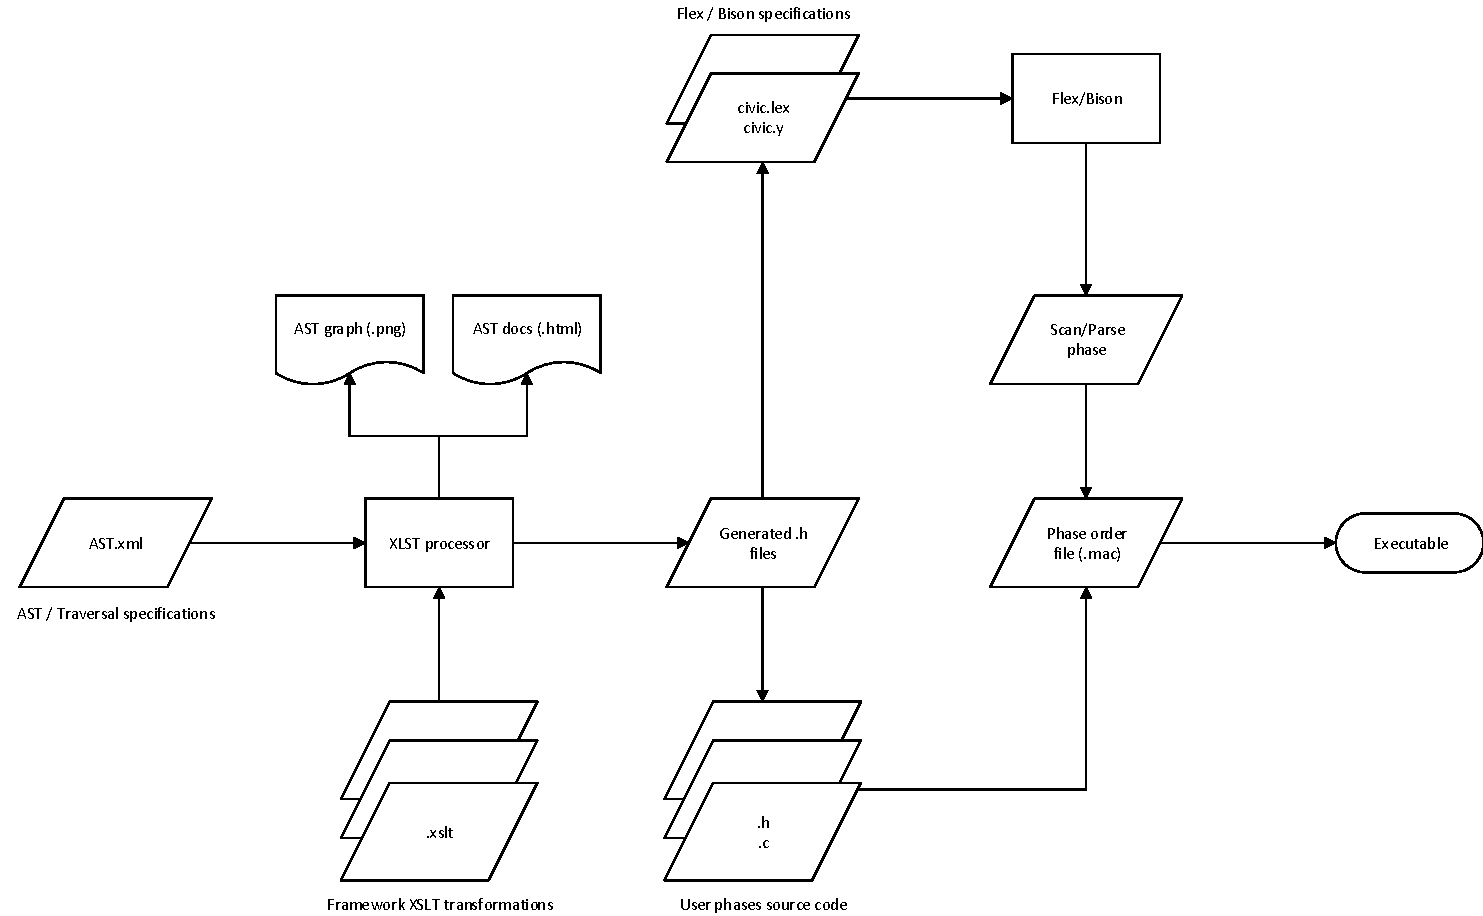
\includegraphics[width=0.95\textwidth]{figures/architecture/overview.pdf}
			\caption{Schematic overview of the Civic framework}
			\label{build-dep}
		\end{figure}
		
		The framework is written in C and XLST and runs on most *nix distributions, provided they support the required packages \footnote{gcc, gzip, flex, bison, xsltproc, dot, indent}. A schematic overview of the architecture is presented in \cref{build-dep}. The framework relies on an XSLT processor to transform a specification of the AST and traverals into C header and source files which can be used by the rest of the compiler. This process is triggered on each build and replaces key files if the specifications are altered.
		
		
	\section{Workflow}
		The framework enforces a specific workflow and code organization structure. It presents the process of compilation as a pipeline of phases, each phase consisting of one or more traversals. Users can modify or expand the pipeline by introducing new phases and traversals, but are bound by this structured approach. Configuration of the pipeline is possible through code and supported by C macro's further explained in the next section. Seperated from code are the specification of the AST and traversal definitions. 
		
		This workflow directs user code largely to:	
		\begin{enumerate}
			\item Specification of AST and traversals (\code{AST.xml})
			\item Traversal header and implementation files (user directory with \code{*.c, *.h} files)
			\item Pipeline configuration file (\code{phase.mac})
		\end{enumerate}
		
		As each compiler requires scanning and parsing, a phase invoking the Flex scanner generator and Bison parser generator are provided by default. While strictly part of bootstrapping code, most users will work with these tools, adding to the above list:
		\begin{enumerate}
			\setcounter{enumi}{3}
			\item Lex configuration for Flex (\code{civic.l})
			\item YACC configuration for Bison (\code{civic.y})
		\end{enumerate}
		
		Changes to the AST or the addition of a new traversal are propagated by building the compiler. The build process produces updated integration code as well as documentation on the AST in two forms: 1) as an HTML document detailing every node and it's children, and 2) as an image depicting the AST graphically, with lines connecting nodes where applicable.
		
		Debugging is assisted through command line arguments which can specify to only compile up to a certain point. In addition, the command line allows configuration of tracer options, which - assuming the user supplemented their code with trace statements - enable detailed output of the callstack.
	
		
	\section{Technical Implementation}
		The most defining characteristic of the framework is the abstraction layer over the AST and traversal mechanisms. To better understand this layer, this section will detail the internal representation of nodes, traversals and phases and discuss the role of code generation. This section assumes knowledge of the C programming section.
		
		\subsection{Abstract Syntax Tree}
			\includexml{node_structure.xml}{xml-node-structure}{Template for specification of a node}
			\includecode{c_node_structure.c}{c-node-structure}{Internal structure of a node}
			
			Nodes in the AST are defined as a \code{<node>} XML element in the \code{<syntaxtree>} element of the \code{AST.xml} specification file. Every node has a name, and optionally a list of named child nodes (or \emph{sons}) and attributes, following the template shown in \cref{xml-node-structure}. The difference between an attribute and a child node is that child nodes \emph{can be traversed}, whereas attributes are simple properties, though they might in fact reference other nodes. The \code{<targets>} element inside either a child or attribute declaration is optional, and is further explained in \cref{tree-validation}.
			
			Internally, nodes are represented by the \code{NODE} structure shown in \cref{c-node-structure}. This structure holds the type of the node as an \code{enum} and references to two union structures representing applicable child nodes and attributes. These structures are generated and union'ed based on the XML specification, which translates a \code{<son>} element to a \code{node*} member of the former and an \code{<attribute>} element to a typed member of the latter. The C-type used for members of the attribute structure comes from a mapping section in the specification.
			
			Besides one being traversible, child nodes and attributes are accessed the same way through generated macro's. These macro's primarily exist to avoid manually selecting which union struct variable should be accessed. A side effect is that it also hides which properties are children and which are attributes, and it implies an attribute cannot have the same name as a child node. Access macro's \emph{do not} ensure they are used on the correct node by validating the node type, as they are used both as a setter on the left-hand side and a getter on the right-hand side, and assignment to condidionals is illegal in C.

		\subsection{Traversals}
			\includexml{trav_structure.xml}{xml-trav-structure}{Template for specification of a traversal}
			
			\begin{figure}
				\begin{lstlisting}[style=xmlstyle,caption=test,label=test2123]
<traversal id="[PFX]" name="[Friendly Name]" default="[sons/user]" include="[header.h]">
	<!-- Element applicable for 'sons' mode -->
	<travuser>
		<node name="[NodeName]"/>
	</travuser>
</traversal>
				\end{lstlisting}
			\end{figure}
			
			Traversals do not have a single, well-defined structure but rather translate into control flow statements and traverse tables. Every AST traversal must be declared in the \code{AST.xml} file as a child of the \code{<phases>} element. All traversals adhere to the template presented in \cref{xml-trav-structure} and require a unique and preferably short prefix, a friendly name, mode of operation and header file with entry points.
			
			Traversals are supported in two modes: 1) user mode and 2) child mode. User mode traversals are required to implement handlers for every node type in the AST, child mode requires only handlers for a specific set of nodes. Every node not on that list is  handled by a catch-all function which automatically traverses child nodes until one a node is found which is specified by the user.
			
			Users can push a traversal onto the stack and request the start of a traversal (snippet \ref{old-arch:start-trav}), triggering a lookup to a table for the active traversal holding the function which should be called index on node type. By default all child nodes are traversed using a switch statement based on node type (snippet \ref{old-arch:switch-trav}). The \code{INFO} struct passed along provides statefulness to receiving functions, though this is not essential for traversal.
			
			On traversals, the mechanism, output generated and implementation
		
		\subsection{Phases}
			Phase.mac file, entry point to traversal
		
		\subsection{Tree Validation}
		\label{tree-validation}
			..
		
	
	\section{Strenghts And Weaknesses}
		....
	
		
		
	\begin{comment}
	\section{Code Generation From XML}
	\label{sec:old-sec}
			One defining characteristic of the framework is an abstraction layer over the AST and traversal mechanisms. To better understand this layer, this section will first summarize how nodes and traversals are internally represented, then detail how the abstraction assists in this process and conclude with a summation of all parts of the framework affected by the layer.
			
			Nodes are stored as a C-struct containing the type of the node and two structures representing their children and attributes (snippet \ref{old-arch:node}). For each node type there are two data structures with it's specific attributes and references to child nodes, the union of which is refered to in the \code{NODE} struct (snippet \ref{old-arch:union}). Access macro's are created for each attribute and child node as well as (de-)allocation code.

			Traversals do not have a well defined single structure but translate into control flow statements and traverse tables. Users can push a traversal onto the stack and request the start of a traversal (snippet \ref{old-arch:start-trav}), triggering a lookup to a table for the active traversal holding the function which should be called index on node type. By default all child nodes are traversed using a switch statement based on node type (snippet \ref{old-arch:switch-trav}). The \code{INFO} struct passed along provides statefulness to receiving functions, though this is not essential for traversal.
			
			To illustrate the complexity involved, consider the introduction of a new node to the AST. To achieve this, every traverse table must be supplemented, the default traverse function must be updated, two new structures must be added to the node union, allocation and de-allocation routines must be written as well as access macro's and the copy, free and check system traversals must be modified. Besides being tedious, performing these tasks manually introduces a significant risk of error. The framework provides XSLT transformations of a specification to automate most of this process. It takes only a couple of lines of XML to add a node to the AST, and all previously mentioned tasks are automatically executed. This does however mean that the specification forming the abstraction is not isolated from the target language (or leaky). For instance, to define a node with a \code{char*} attribute requires the specification to know about the difference in copying C-strings and integers.
					
			Specifications and accompanying translations are given for:
			\begin{itemize}
				\item Nodes which form the abstract syntax tree, along with their applicable attributes and child nodes
				\item Mapping from friendly attribute names to C-types, and relevant methods used for copying and free-ing
				\item Node constraints on:
				\begin{itemize}
					\item Type: only certain child nodes or attribute are valid
					\item Requirement: attributes or child node must be present
					\item Applicable phase: some attributes are not always required
				\end{itemize}
				\item Traversals, their mode of operation, affected nodes and function prefix
			\end{itemize}
		
	\section{Flexible Traversals}
			Internals of the traversal have been briefly shown in section \ref{sec:old-sec} and will be explained in more detail in this section. 
			
			Traversals are supported in two modes: 1) user mode and 2) child mode. User mode traversals are required to implement handlers for every node type defined in the AST, child mode requires only handlers for a specified list of nodes. Every node which is not on the user specified list is routed instead to a catch-all function which automatically traverses child nodes of the unhandled node. This function is automatically updated when a node is added or removed or a change is made to any of the child node properties.
			
			All traversals are elements in the \code{<phases>} element of the specification document, and must contain a unique identifier, readable short name, operation mode (user or child), associated header file and - depending on the chosen mode - a list of nodes handled by the traversal. When the compiler is built, enumerations of all node and traversal identifiers are generated. All nodes and traversals are assigned a zero-indexed integer to be used as an index. Every traversal adds an array of function pointers to the traverse table. The row is added at the index dictated by the enumeration and the array is indexed by the node index. References to the funtions are constructed by concatenating the traversal identifier with the friendly name of the node. In child mode, unhandled node types are routed to the catch-all function explained in the last paragraph.
			
			Every handler has the same function signature, requiring pointers to a node and an info structure, and returning a pointer to a node which replaces the current node. If a traversal is to be used as an entry point for a sub-phase, it must be added to the \code{phase.mac} file, where an entry point is referenced with the same signature as a handler function: \\
			\code{node *PFXnodeType (node *arg\_node, info *arg\_info)}
						
			The framework maintains a stack of active traversals manipulated with the \code{TRAVpush (id)} and \code{TRAVpop ()} functions. An active traversal can be controlled with the \code{TRAVdo (node*, info*)}, \code{TRAVopt (node*, info*)} and \code{TRAVcont (node*, info*)} functions. All return the result of the traversal of a given subtree, additionally the latter two respectively ignore null node arguments and invoke the catch-all handler.
			
			This approach to traversals encourages users to create small, reusable traversals in similar way the visitor pattern is implemented in an object-oriented language \cite{gof1994}.
			
	\section{Tree Validation}\label{sec:validation}
			As explained in section \ref{sec:old-sec}, nodes all share the same structure. Semantically all node structures are valid trees, yet most combinations of AST nodes should yield an invalid tree. This section briefly explains the validation mechanisms present in the framework.
			
			The first line of defense against illegal node operations is the tagged union implemented for nodes. A tagged union is a structure which can take on different but fixed types \cite{unknown}. An \code{enum} is used to distinguish all different node types and used in the generated traversals to always pick the correct structure when traversing. Unlike functional languages, C provides no compile time checks to enforce the tagged union except for a simple check on the node type. However, access to nodes and traversal mechanisms are largely controlled from generated macro's which do provide a level of security. It must be noted that the macro property accessors do not check the node type, as they are used on both the left- and righthand side of assignments and assignments to conditionals are illegal in C.
			
			The main validation mechanism lies in the 'check' traversal generated from the AST. This traversal walks the AST and ensures that every node has child nodes and attributes of the correct type, and that any attribute or child node marked as mandatory for the current phase is present. The check traversal must be manually added as part of a phase, so invalid trees are still possible during execution of any traversal up to the check. 
		
	\section{Development Environment}
		Todo:
		\begin{itemize}
			\item Error handling
			\item Pre-configured scanner, parser
			\item Debug helpers
			\item Compact base library
		\end{itemize}
	\end{comment}
	
	
	
\chapter{Re-design: Code Over Specification}
	This chapter approaches the framework described in the previous chapter from the perspective of a modern object-oriented language.

	Modern language, infrastructure approach, type-safety, code-based AST. Key questions:
	\begin{itemize}
		\item Which programming languages are realistic alternatives to the current language, keeping in mind the current experience of students?
		\item Which areas or concepts could be improved or introduced to improve the framework's efficiency?
		\begin{itemize}
			\item In what way are these concepts dependent on implementation language or on choice of architecture?
			\item Which concepts are invariant of platform or architecture?
		\end{itemize}
	\end{itemize}
	
	In theory the existing architecture could be re-used with the code generator outputting C\# instead, cleaner strategies exist which will be discussed in this section. The applicability of an abstractian layer will be tested by developing a model for a type-safe AST, followed by a proposal for a code-configured pluggable architecture.
		
		Fundamentally changed:
		- language choice
		\begin{itemize}
			\item Code-First vs specification (for AST, traversals and phases - also validation omitted)
			\item Managed Language
			\item Package updates
		\end{itemize}
		Untouched or adapted:
		\begin{itemize}
			\item Traversal Mechanism (added lambda)
			\item Collection representation
			\item Base lib (arguments, default ANTLR4, documentation)
		\end{itemize}
	
	\section{Language Selection}
		While C is arguably as modern and widely used as any other general purpose programming language, and can even be called object-oriented \cite{book:schreiner}, it is definiatly not strongly typed. Programming in C requires defensive programming and dynamic type casts to achieve a level of safety other languages get for free, as internally every structure is a \code{void*}. In this section the language options for a modernized Civic framework are briefly discussed.
		
		Choosing a language is a non-trivial task and depends on many factors. For this project, the first criteria was that the language must be high-level and preferably managed to reduce the time spent debugging memory allocation and null references in C. Student familiarity with the language was also considered, as well as the exclusion of any fully functional languages. The reason for the latter being removal of the functional programming course from the undergraduate program. One final consideration was the availability of relevant libraries and support infrastructure. 
		
		With functional languages excluded, procedural and scripting languages remain. A recent study found the most common languages on GitHub in these categories to be C++, C\#, Objective-C, Java, Go, JavaScript, Python, Perl, Php and Ruby \cite{Ray2014}. A study by \citeauthor{Meyerovich2013} found that 97\% of computer science majors knew at least one imperative/OO language against 78\% for dynamic languages \cite{Meyerovich2013}. Studies on static versus dynamic typing are somewhat inconclusive, though evidence suggests static typing improves maintainability, increases understanding of undocumented code and measurably reduces defects \cite{Hanenberg2014,Ray2014}.
		
		When considering only statically typed managed languages, only C\#, Java and Go remain. The TIOBE index is a  programming language popularity index based on the number of hits in various search engines. While Java and C\# occupy position 3 and 6 respectively, Go takes the 30th place, just below Ada \cite{Nanz2014}. With both C\# and Java able to use the LL(*) ANTLR4 parser generator, either of these languages would suit the project.
		
		Todo:
		\begin{itemize}
			\item C\# has more powerful semantics, lambdas, properties, optional dynamic typing
			\item But it is somewhat plaform bound, whereas Java is not
		\end{itemize}
						
	\section{Type-Safe AST}
	\label{sec:type-safe-ast}
		Working with a strongly typed OO-language grants the ability to model AST nodes in greater detail than before. Different node types can be represented by different classes with node specific attributes exposed as properties, sharing a common interface or base class which can be used in traversals. Child nodes on a node should also be strongly typed and accessible in the same way as attributes. This poses an interesting challenge: if traversible properties are placed on the derived class, how can a traversal operating on the base class access them?
		
		Two possible solutions come to mind: the first one - used in the existing framework - is to supplement the traversal with knowledge of the traversible properties, resulting in large switch statements. The second option is to mark traversible properties with an attribute (in Java attributes are known as annotations) and use reflection to retrieve them at runtime. A basic working version is shown in snippet \ref{reflection-base-simple}. A note for those unfamiliar with C\#, the \code{\{ get; set; \}} represent an automatic property, similar to simple field-backed get/set methods in Java. The \code{.Where(p => p...)} method call on line 23 is an example of a lambda filter applied to all elements returned from \code{GetType().GetProperties()}, the \code{.Any(att => att..)} clause inside the lambda returns a boolean if any of the attributes declared on a property match the nested expression.
			
		This basic setup fails on several counts. First of all, the order in which properties are declared on a class is not guaranteed to match the order in which they are returned from reflection. Second, it is possible to place the \code{[Child]} attribute on any attribute which is then added to the list of traversible children. C\# 4.5 exposes declaration information via attributes, which is used to populate a field on the attribute. This order can be used to sort the list of properties, as shown in snippet \ref{reflection-base}.
				
		The \code{Node} abstract base class and the \code{ChildAttribute} attribute form the basis of the approach chosen for a type-safe AST. Nodesets from the previous framework can be exchanged for (abstract) base-classes for easy targeting of expressions, statements, or variable declarations. Because C\# (and Java) only support single-inheritance, a node is limited to only one branch of inheritance, which is probably a good thing.\footnote{An effort has been made to implement a object composition model, which required too much documentation to explain and provided identical results.}
	
		It must be noted that the order in which child properties are returned is somewhat ambiguous when working with an inheritance hierarchy where traversible properties are defined on multiple classes. Properties are correctly retrieved, but are sorted on line number, which is valid only for a single file. This poses a problem for classes defined over multiple files. This behavior is arguably undefined, though such a list might be ordered first by order of inheritance, and then by line number. Sorting this way is non-trivial and unnecessarily costly, considering there were no real use cases for such hierarchies, so no action was required.
					
	\section{Improved Traversal Mechanisms}
		This section reviews common traversal and manipulation mechanisms applicable for trees with nodes in an inheritance tree and presents three traversal mechanisms for the type-safe AST. The section concludes with the benchmarking and optimization of the general purpose visitor and the lambda-based visitor. 
				
		In the analysis of the existing framework the traversal mechanism was identified as some form of visitor pattern. The visitor pattern was first formally defined by \citeauthor{gof1994} in 1994, who defined its intent as: ``Represent an operation to be performed on the elements of an object structure. Visitor lets you define a new operation without changing the classes of the elements on which it operates.''. Parallels with the requirements for the traversal mechanism on an AST are easily drawn, coincidentally the one example they present is \emph{about a fictional AST}! To quickly summarize the example, instead of seperating compilation phases into logical units, functionality is placed in a method accessible on \emph{every} node. Thus, the type checking phase would add an overridable \code{TypeCheck ()} function to the base class, and responsibility for traversing child nodes is placed on the node as well.
		
		The visitor pattern disapproves the modification of a node class for every new operation on a tree. It defines a \code{NodeVisitor} base class which contains a visit method for every node in the hierarchy (\code{VisitAssignment(AssignmentNode)}, \code{VisitDeclaration(Declaration)}, etc). A method accepting the visitor class is added to every node (\code{Accept(NodeVisitor)}), whose sole purpose is to return control to the visitor class by calling the visit method for that node. Each new operation of the tree results in a derived visitor containing only the relevant functionality.
		
		The classic example of the pattern is not shown here, as it only demonstrates unwanted code. The main design goals for the upcomming three visitor implementations are a maximumum reduction of clutter and a transparant algorithm. Less clutter means faster or at least more time spent on actual development and should everything go wrong, it should at least be clear where it goes wrong.
		
		\subsection{View-Only Visitor}
			The first algorithm presented traverses an AST as defined in section \ref{sec:type-safe-ast} and invokes publicly defined \emph{Visit(...)} methods on the class. This scenario most closely resembles the default visitor pattern adapted for reflection. As anticipated in the design of the AST, a reflection based visitor requires meta-information on which properties are traversible and in what order. Access to child properties is provided by the \code{Node.ChildProperties} property, which returns a read-only list of child properties. Traversal of children is performed by the \code{VisitChildren()} method, which closely resembles a reflection based version of the catch-all function in the C-based framework. 
			
			The view-only visitor is presented in snippet \ref{readonly}. Unbeknownst to the author of this paper, a generalized version of the visitor pattern titled \emph{Walkabout} was presented in 2007 by \citeauthor{palsberg1998essence}. The algorithm is (unsurprisingly) identical in form, and may be easier to follow if unfamiliar with C\# (see snippet \ref{walkabout}).
		
		\subsection{General Purpose Visitor}
			Transformations often require the replacement of nodes with nodes of another type but with a common ancestor. In this section the view-only visitor is modified to support node replacement.
			
			The flexibility found in the C-based traversal can be applied to the view-only visitor by adding return values to visitor handlers. It is important to realize that a transformation from type A to type B is not always applicable, even if they share a common ancestor. The reason for this is that every node in the tree is bounded by the type of the property. Thus, if a type A node is held in a property of type A, replacing it with a type B node would cause a runtime exception or compilation error and should be prevented.
			
			An additional parameter is required on the generic visitor function which can be used internally by the  \code{VisitChildren()} method to pass the enclosing type of the propererty. Consumers of the visitor should not need this type parameter, as they only invoke the generic visitor if no overload in their implementation matches, in which case the maximum upcast is as it was before, the generic type parameter. The general purpose visitor is presented in snippet \ref{gen-visit-changes}.
			
			This visitor is able to deal with out-of-bound handlers by utilizing two mechanics: 1) user code directly invoking the unfit handler won't compile because of static type checking and 2) automatic child traversal or forced invocations of the generic visitor are properly bound to a safe limit.
			
			One final test remains, what happens when multiple matching handlers are defined? It is possible to write a handler for a base type as well as one for a concrete type. For automatic traversals, the most derived handler is automatically chosen because the runtime type if always used for method selection. However, user code is bound to the single-dispatch mechanism which selects a method is based on the type of the \emph{reference} holding the object. A derived type inside a variable of the base type will be routed to to the base type handler.
			
			This is not as bad as it seems as pre-compile inspection will show which method will be invoked. If this behavior is unwanted, the argument to the visitor function can be dynamically cast to delay method selection until runtime (since C\# 4.0 \cite{schildt2010c}). 
			
			This leaves two unsupported cases:
			\begin{enumerate}
				\item Two or more handlers differing only in return type
				\item Two or more handlers, where the derived handler returns a more generic type than the less derived handler
			\end{enumerate}
			
			The first one is an illegal construct in C\# and most other imperative languages which cannot be avoided. The second one is a result from reliance on the \code{Type.GetMethod(...)} function to choose a function based on the first argument. This matching process is done without accounting for suitable return type, so if the most derived guess fails the second test, no other options are evaluated. Solving this issue means a full implementation of multiple-dispatch, which is preferably avoided.
			
		\subsection{Lambda Visitor}
			While the general purpose visitor is sufficient for most traversals, it requires some care when multiple layers of an inheritance hierarchy are targeted. Method invocation depends on two seperate mechanisms (single-dispatch and reflection), one of which is not very flexible. As an alternative to a full multiple-dispatch implementation, this section will discuss the lambda visitor, which removes publicly defined method alltogether.
			
			Eliminating single-dispatch means replacing the publicly defined visitor handlers with an ordered list of delegates and configuration functions to modify the list. The basic traversal mechanism remains the same, but instead of probing for publicly exposed methods the list of handlers is consulted instead. Multiple-dispatch related ambiguity with targets across multiple layers of inheritance is solved by explicitly stating the order of evaluation. Such handlers must contain at least:
			\begin{enumerate}
				\item Type of the node handled
				\item Return type of the handler
				\item Delegate containing the transformation function
			\end{enumerate}
			
			The distinction previously made between replace method and 'view-only' methods can be removed by offering two types of delegates. In .NET these are represented by the \code{Func<TArg, TRet>} and \code{Action<TArg>}  delegates, indicating respectively a function which takes an object of type TArg and returns an object of type TRet and a function which takes an object of type TArg but doesn't return anything (void function). These can be interleaved as in returning nothing in the context of tree traversals indicates ``no change'' to the initial object; it would behave as if it would return itself.
			
			The logic determining which handler should be invoked is now entirely encapsulated by the visitor, a simple but useful feature would be an optional predicate preceding invocation of the function. This, together with a lambda-style approach to defining visitor methods allows for more configuration flexibility. Such handlers must additionally hold:
			\begin{enumerate}
				\setcounter{enumi}{3}
				\item Delegate type (void or returns)
				\item Delegate containing a predicate
			\end{enumerate}
						
			Additionally, fall-through handlers could be supported with this approach, though the decision not to do so is based on the fact that fall-through statements have been mostly expelled from switch constructs in modern languages as they are a frequent cause of bugs. A documented version of the lambda visitor is presented in snippet \ref{lambda}.
			
		\subsection{Benchmarks \& Optimization}
			The two traversal mechanisms compared in this section are the general purpose visitor and the lambda-visitor. A small benchmark suite has been developed which provides somewhat realistic data structures and can easily run tests on any number of visitor implementations. The view-only visitor was not included as it does not perform the same tasks as the other two.
			
			First of all realistic test data must be produced. Part of the unit test suite included in the library of the framework provides static methods which generates small trees from a 10-node AST. Abstract classes are used as markers and the diversity of the nodes meets the criteria used in unit tests making them suitable for use in a benchmark suite.
			
			The idea is to start with a small tree (n=14) with three layers of depth, and perform replacements with the same tree on certain blocks, providing a growth factor of roughly 5.5. After 4 iterations of the visitor the tree will have grown to 12098 nodes, which is likely below the limit where memory allocation starts to play a major role and above the threshold for measurable differences.
			
			The first test run with 250 iterations, repeated 3 times produced the results shown in figure \ref{fig:first-run}. Well, at least the performance impact of the \code{DynamicInvoke(...)} call are not quite as significant as some sources proclaim \cite{website:msdn-reflection}. It does beg the question if the results should be explained by a largely similar algorithm, or if there is another bottleneck in the system.
			
			The tests were run again and profiled using an educational copy of the JetBrains dotTrace profiling software. The number of iterations was brought down to 200 and the number of tries to 1. After 50 seconds the results were in: 42 seconds were spent inside in the system libraries on 700 million library calls. A mere 6 seconds were spent on all benchmarking code (responsible for 5.5 million node creations 30 million fixture calls), and less than a second was spend on garbage collection. The culprit was quickly identified: over 3 million cold calls were made to the extension method which enumerates the properties on a type which have the child attribute. These lists were cached, but on the objects themselves; perhaps a static dictionary is better suited. The results were drastic: the profiler ran in only 1.9 seconds, a reduction of factor 20. The first run was repeated and saw an factor 10 reduction in runtime (figure \ref{fig:second-run}).
												
			\begin{figure}
				\centering
				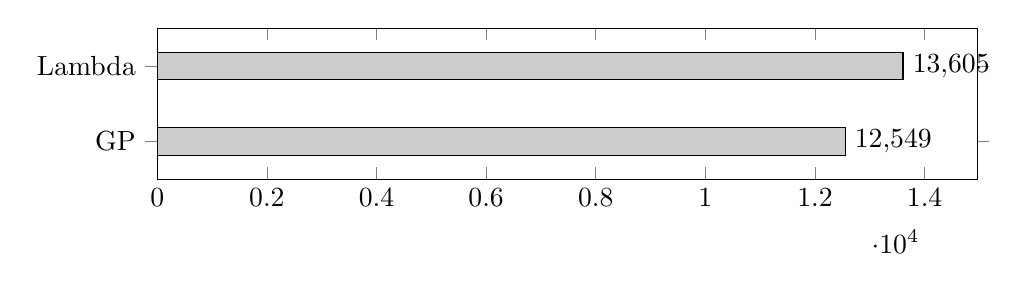
\begin{tikzpicture}
				\begin{axis}[
					xbar, xmin=0,
					width=12cm, height=3.5cm, enlarge y limits=0.5,
					symbolic y coords={GP,Lambda},
					ytick=data,
					nodes near coords, nodes near coords align={horizontal},
				]
				\addplot[fill=lightgray] coordinates {(12549,GP) (13605,Lambda)};
				\end{axis}
				\end{tikzpicture}
				\caption{Initial run - \emph{avg. miliseconds per run}, \emph{iters}=250, \emph{n}=3}
				\label{fig:first-run}
			\end{figure}
			
			\begin{figure}
				\centering
				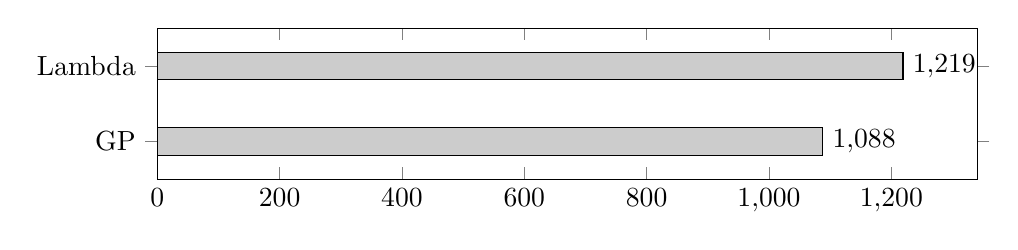
\begin{tikzpicture}
				\begin{axis}[
					xbar, xmin=0,
					width=12cm, height=3.5cm, enlarge y limits=0.5,
					symbolic y coords={GP,Lambda},
					ytick=data,
					nodes near coords, nodes near coords align={horizontal},
				]
				\addplot[fill=lightgray] coordinates {(1088,GP) (1219,Lambda)};
				\end{axis}
				\end{tikzpicture}
				\caption{Second run - \emph{avg. miliseconds per run}, \emph{iters}=250, \emph{n}=3}
				\label{fig:second-run}
			\end{figure}
			
				
	\section{Pluggable Architecture}
		- XSLT not necessary for AST generation, or check/copy travs (present copy function)
		
		Phases reduced to list of traversals, as there is no need for logical seperation.
		- phases defined with interface, code-based configuration of phases (optionally based on console arguments)
		- grouping easy to add if required
	
	
	\section{Collections}
		While an AST as defined in section \ref{sec:type-safe-ast} has more depth than what was previously possible, it is still the same basic tree structure as before. One area which could be improved is in the representation of a collection of nodes. A function may have an arbitrary number of parameters, variables, nested functions and statements, is it possible to represent these structures more clearly with built-in lists?
		
		\begin{figure}[ht]
			\begin{minipage}[b]{0.45\linewidth}
				\centering
				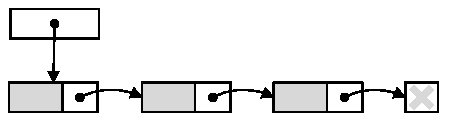
\includegraphics[width=\textwidth]{figures/collections/sll}
				\caption{Singly linked list}
				\label{fig:sll}
			\end{minipage}
			\hspace{0.5cm}
			\begin{minipage}[b]{0.45\linewidth}
				\centering
				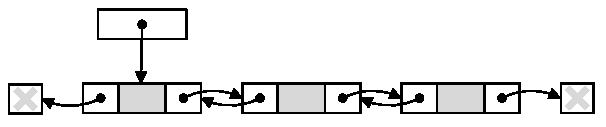
\includegraphics[width=\textwidth]{figures/collections/dll}
				\caption{Doubly linked list}
				\label{fig:dll}
			\end{minipage}
		\end{figure}
		\begin{figure}[h]
			\centering
			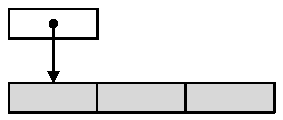
\includegraphics{figures/collections/list}
			\caption{Dynamic array or list structure}
			\label{fig:list}
		\end{figure}
		
		A variable number of nodes is implemented in an AST by nesting container nodes up to the depth required, forming either a singly-linked list (fig. \ref{fig:sll}) or a doubly-linked list (fig. \ref{fig:dll}). A node holding any number of child nodes might be represented in C\# as in snippet \ref{fig:col-sample}.

		\includecode{lists_as_attribs.cs}{col-sample}{Example of lists as traversible attributes}		
	
		This poses the question how such a list should be treated. I should we see a list of nodes as a special type of node with no traversible children but traversible or can the functionality  \code{ChildAttribute} defined in section \ref{sec:type-safe-ast} 
		
		Case with collections:
		- Node child may be node (or derived) or list of nodes
		- Discriminated union in C\# (https://stackoverflow.com/questions/3151702/discriminated-union-in-c-sharp)
		- What doesn't work: Every node is also a list of nodes
		- Cyclic dependency in inheritance (Node : IList?)
		- Advantages: easy to add, iterate and replace
		- Disadvantages: Traversal issues (can a handler return a list?), complicates everything
		
		Case without collections:
		- More natural to traversals
		- Singly-linked or doubly-linked
		- Difficult to append to or modify
		- Can be overcome with extension methods
		
		Outcome: chosen for no collection types in lists, to avoid confusion with traversals.
			
	\section{Development Environment}
		Implications of unmanaged vs managed, reduction of base library, debug upgrade..?
		
		\subsection{Updated Lexer/Parser}
			More flexible Parser/Lexer generator support, such as ANTLR4 (LL(*) with EBNF).
						
			Language dependency: Plenty of parsers exist for any language, first version of AST most likely constructed in code; change of language not essential.
			
			Platform dependency: Depends on extensibility of parser generator, ANTLR4 has multiple ways of traversing a generated parse tree, YACC does not (embedding of code in parse phase restricts construction of AST)
			
		\subsection{Platform Updates}
			NuGet
			
		\subsection{Documentation Generator}
			Inheritance graph plotter, AST graph plotter
	
	\section{Validation}
		Type-safety is more than enough?
		
		Old method was not type safe, simply prevented untracable errors
		
		Tree corruption unnoticed until check routine ran
		
		Classes as f
	
\chapter{Discussion}
	vNext immutable AST, 
	
	Language choice, developers switch language often
		We found that developers rapidly and frequently learn
		languages. Factors such as age play a smaller role than suggested
		by media. In contrast, which languages developers
		learn is influenced by their education, and in particular, curriculum
		design.
		
	Functional
		Promisingly, developers who learned a functional or	math-oriented language in school are more than twice as likely to know one later than those who did not.
		
\chapter{Code Samples - To Remove}
	\includecode{c_node_union.c}{old-arch:union}{Sample child node and attribute union structures for node}
	\includecode{c_init_trav.c}{old-arch:start-trav}{Starting a traversal}
	\includecode{c_trav_sons.c}{old-arch:switch-trav}{Excerpt from catch-all switch construct}
	\includecode{ast1.cs}{reflection-base-simple}{Using reflection to retrieve marked properties from a derived class}
	\includecode{ast2.cs}{reflection-base}{Updated code for the base class and attribute}
	\includecode{walkabout.java}{walkabout}{Walkabout algorithm by \citeauthor{palsberg1998essence}}
	\includecode{viewonly.cs}{readonly}{View-only visitor}
	\includecode{gen_visitor.cs}{gen-visit}{Generalized visitor}
	\includecode{lambda_visitor.cs}{lambda}{Lambda-based visitor}	

\bibliography{report}
\bibliographystyle{plainnat}
\end{document}